\newlength{\bibsep}
\documentclass[nonatbib,5p,a4paper]{elsarticle}
\usepackage[english]{babel}
\usepackage[DatePublished]{code/style}
\usepackage{csquotes}
\usepackage{lipsum}
\usepackage{amsmath}
\usepackage{physics}
\usepackage{cuted}
\usepackage{derivative}
\selectlanguage{english}
\usepackage{tikz}
\usetikzlibrary{decorations.pathmorphing}
\usepackage{newfloat}
\usepackage{multicol}
\usepackage[section]{placeins}

\DeclareFloatingEnvironment[fileext=lof]{graph}[Graph][List of Graphs]

\let\oldsqrt\sqrt
\def\sqrt{\mathpalette\DHLhksqrt}
\def\DHLhksqrt#1#2{%
\setbox0=\hbox{$#1\oldsqrt{#2\,}$}\dimen0=\ht0
\advance\dimen0-0.2\ht0
\setbox2=\hbox{\vrule height\ht0 depth -\dimen0}%
{\box0\lower0.4pt\box2}}

\makeatletter
\newcommand*{\overrightharpoonup}{\mathpalette{\overarrow@\rightharpoonupfill@}}
\newcommand*{\rightharpoonupfill@}{\arrowfill@\relbar\relbar\rightharpoonup}
\makeatother

\DeclareFontFamily{U}{matha}{\hyphenchar\font45}
\DeclareFontShape{U}{matha}{m}{n}{
      <5> <6> <7> <8> <9> <10> gen * matha
      <10.95> matha10 <12> <14.4> <17.28> <20.74> <24.88> matha12
      }{}
\DeclareSymbolFont{matha}{U}{matha}{m}{n}
\DeclareMathSymbol{\varrightharpoonup}{3}{matha}{"E1}
\let\rightharpoonup\varrightharpoonup
\newcommand*{\vect}{\overrightharpoonup}

\addbibresource{bibliography/sources.bib}

\begin{document}

\begin{frontmatter}

\title{%
\textbf{Factors Affecting the Damping Constant of a Spring System}\\
\small Submitted for assessment in 12A\_PHY1
}

\author{James Bray} 
\address{Christ Church Grammar School}

\newdate{dateName}{2}{09}{2025} % edit the date here, ' dateName ' has to match on these two lines.
\renewcommand*{\today}{\DayMonthYearDateFormat\displaydate{dateName}} 

\NameOfAbstract{Abstract}
\begin{abstract}

\lipsum[0-1]

\end{abstract}

\end{frontmatter}
\begin{figure}
    \centering
    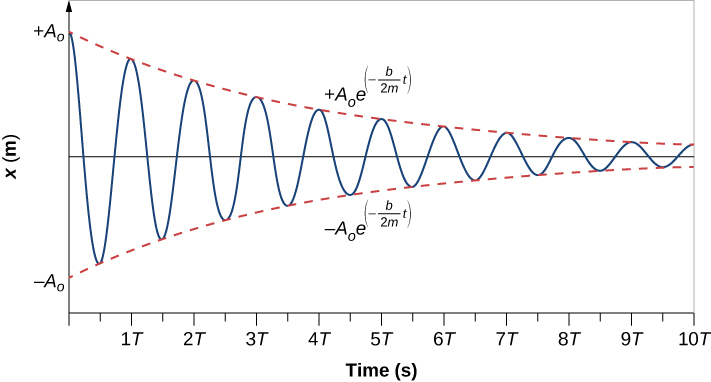
\includegraphics[width=0.47\textwidth]{images/damped_shm.png}
    \caption{Displacement--time graph illustrating the characteristics of an underdamped harmonic oscillator.}
\end{figure}

\section{Introduction}

A vertical mass--spring system provides a simple model for studying oscillatory motion and energy dissipation in mechanical systems. An ideal mass--spring system undergoes simple harmonic motion with constant amplitude, but in real conditions mechanical energy is dissipated through a variety of means, causing oscillations to gradually decrease in amplitude. This phenomenon is known as damping, defined as "the loss of energy of an oscillating system by dissipation."

The degree of damping can be characterised by the decay constant $\gamma$, which specifies the rate at which oscillations diminish; larger values correspond to faster energy loss and more rapid amplitude reduction. The value of this constant depends on both the properties of the oscillating mass and the restoring system.

\subsection{Aim and Hypothesis}
The aim of this investigation is to determine how spring configuration and attached mass influence the rate of damping, quantified by the exponential decay constant $\gamma$, in a vertically oscillating mass-spring system.

It is hypothesised that if the attached mass is increased, there will be a decrease in the decay constant $\gamma$ proportional to $m{\textsubscript{load}}^{-1}$, and if the spring system is configured in series, there will also be a decrease in the decay constant.

The primary sources of damping are expected to be internal friction within the spring in conjunction with resistive forces such as air drag on the mass. For simplicity, it will be assumed that these factors can be modelled by a damping force which is linearly dependent on velocity, as with a standard viscous dampening model.

\subsection{Variables}
\begin{description}
    \item[{\small\bfseries Independent Variables:}] The mass of the load attached to the end of the spring, and the configuration of the spring system.
    \item[{\small\bfseries Dependent Variable:}] The curve-fitting coefficients of the damped harmonic motion displacement-time graph.
    \item[{\small\bfseries Controlled Variables:}] The positioning of the retort stand and clamps, motion sensor alignment and sampling frequency, mass cross-sectional geometry, and ambient air conditions (temperature, pressure, humidity).
\end{description}
\clearpage
\section{Theory}

\lipsum[30-36]
\clearpage
\section{Method and Equipment}

\lipsum[4-5]

\section{Results}

\lipsum[5-6]

\setlength{\tabcolsep}{4pt} % default ~6pt
\begin{table}[!ht]
	\caption{Regression parameters for the light spring.}
    \centering
    \begin{tabular}{|
        S[table-format=1.5,table-number-alignment=center] !{\vrule width 1.2pt}
        S[table-format=1.5] |
        S[table-format=1.5] |
        S[table-format=1.2] !{\vrule width 1.2pt}
        S[table-format=1.4] |
    }
    \hline
    \rowcolor{lightgray}
    {$m{\textsubscript{load}}$} & {$A$} & {$\gamma$} & {$\omega'$} & {$R^2$}\\
    \rowcolor{lightgray}
    {(\si{\kilo\gram})} & {(\si{\meter})} & {(\si{\per\second})} & {(\si{\radian\per\second})} & {}\\
    \hline
    0,05025 & 0,01133 & 0,02424 & 21,47 & 0,9990 \\
	0,10014 & 0,01220 & 0,01752 & 15,43 & 0,8385 \\
	0,15044 & 0,02408 & 0,01478 & 12,53 & 0,9947 \\
	0,20011 & 0,04302 & 0,01326 & 10,89 & 0,9996 \\
	0,25019 & 0,04420 & 0,01224 & 9,75 & 0,9894 \\
	0,30012 & 0,11210 & 0,01183 & 8,92 & 0,9999 \\
	0,34991 & 0,13050 & 0,01138 & 8,28 & 0,9999 \\
    \hline
    \end{tabular}
    \label{tab:lightspring}
\end{table}

\begin{table}[!ht]
	\caption{Regression parameters for the stiff spring.}
    \centering
    \begin{tabular}{|
        S[table-format=1.5,table-number-alignment=center] !{\vrule width 1.2pt}
        S[table-format=1.5] |
        S[table-format=1.5] |
        S[table-format=1.2] !{\vrule width 1.2pt}
        S[table-format=1.4] |
    }
    \hline
    \rowcolor{lightgray}
    {$m{\textsubscript{load}}$} & {$A$} & {$\gamma$} & {$\omega'$} & {$R^2$}\\
    \rowcolor{lightgray}
    {(\si{\kilo\gram})} & {(\si{\meter})} & {(\si{\per\second})} & {(\si{\radian\per\second})} & {}\\
    \hline
    0,30010 & 0,03017 & 0,00777 & 13,41 & 0,9971 \\
	0,35014 & 0,04513 & 0,00654 & 12,45 & 0,9955 \\
	0,40014 & 0,05404 & 0,00595 & 11,67 & 0,9993 \\
	0,45004 & 0,06417 & 0,00535 & 11,02 & 0,9993 \\
	0,49984 & 0,06948 & 0,00491 & 10,47 & 0,9995 \\
    \hline
    \end{tabular}
    \label{tab:stiffspring}
\end{table}

\begin{table}[!ht]
	\caption{Regression parameters for two stiff springs in series.}
    \centering
    \begin{tabular}{|
        S[table-format=1.5,table-number-alignment=center] !{\vrule width 1.2pt}
        S[table-format=1.5] |
        S[table-format=1.5] |
        S[table-format=1.2] !{\vrule width 1.2pt}
        S[table-format=1.4] |
    }
    \hline
    \rowcolor{lightgray}
    {$m{\textsubscript{load}}$} & {$A$} & {$\gamma$} & {$\omega'$} & {$R^2$}\\
    \rowcolor{lightgray}
    {(\si{\kilo\gram})} & {(\si{\meter})} & {(\si{\per\second})} & {(\si{\radian\per\second})} & {}\\
    \hline
    0,30010 & 0,07161 & 0,00496 & 9,581 & 0,9996 \\
	0,35014 & 0,09685 & 0,00432 & 8,907 & 0,9995 \\
	0,40014 & 0,1114  & 0,00347 & 8,363 & 0,9991 \\
	0,45004 & 0,1214  & 0,00311 & 7,907 & 0,9995 \\
	0,49984 & 0,1385  & 0,00279 & 7,517 & 0,9996 \\
    \hline
    \end{tabular}
    \label{tab:seriesstiffsprings}
\end{table}
\nopagebreak
\section{Analysis of Results}

\lipsum[6-15]
\section{Evaluation}
\setlength{\parindent}{15pt}

A significant systematic source of error in this investigation arises from neglecting the mass of the spring itself. The oscillating system’s effective mass is not only from the attached load but includes a portion of the spring’s mass, typically approximated as $m_{\mathrm{equ}} = m_{\mathrm{load}} + \tfrac{1}{3} m_{\mathrm{spring}}$. Failure to account for this results in an overestimation of $\gamma$ for a given $m_{\mathrm{load}}$, particularly for lighter loads where the spring mass constitutes a larger fraction of the total oscillating mass. The impact can be quantified as shown below, demonstrating that neglecting the spring mass reduces the accuracy of the measured gradient in $\gamma$ versus $m_{\mathrm{load}}^{-1}$. To mitigate this, future analyses should explicitly include the spring’s contribution to the effective mass in all calculations, ensuring that calculated parameters more accurately reflect the actual system values.

\vspace{-1em}

\begin{align*}
\intertext{Let $m_{\mathrm{equ}} = m_{\mathrm{load}} + \tfrac{1}{3} m_{\mathrm{spring}}$ and $\lambda = m_{\mathrm{load}}^{-1}$}
\gamma &= \frac{b}{2 m_{\mathrm{equ}}} \\
       &= \frac{b}{2 \left(m_{\mathrm{load}} + \tfrac{1}{3} m_{\mathrm{spring}}\right)} \\
       &= \frac{b}{2 \left(\tfrac{1}{\lambda} + \tfrac{1}{3} m_{\mathrm{spring}}\right)} \\
       &= \frac{b}{2} \frac{\lambda}{1 + \tfrac{1}{3} m_{\mathrm{spring}} \, \lambda} \\
\therefore \frac{d \gamma}{d \lambda} &= \frac{b}{2} \frac{1}{\left(1 + \tfrac{1}{3} m_{\mathrm{spring}} \, \lambda\right)^2}
\end{align*}

\vspace{0.5em}

\noindent This form shows that the true relationship between $\gamma$ and $\lambda$ is not perfectly linear, with the denominator introducing a slight downwards concavity.
A straight-line fit that assumes $\tfrac{1}{3} m_{\mathrm{spring}} = 0$ therefore introduces a systematic error that always leads to an underestimation of $b$ for a constant $\gamma$.

Graphically, this appears as a decreased gradient when plotting $\gamma$ against $m_{\mathrm{load}}^{-1}$ and a slight non-linearity, particularly at lower masses. Correcting for spring mass would both steepen the slope and improve linearity, yielding more accurate estimates of $b$ from the decay constant.

Random errors also affected the investigation, particularly due to environmental and material factors. Uncontrolled air resistance introduces variability in the observed amplitude decay, reducing precision in the determination of $\gamma$ across repeated trials. This can be minimised by conducting the experiment in a closed environment or vacuum chamber, thereby stabilising external forces acting on the oscillating mass. Additionally, plastic deformation of the springs over repeated oscillations alters their effective spring constants between trials, introducing both random and systematic deviations in measured $\gamma$ and $\omega'$. Using springs made from metals with low plasticity or replacing springs with near-perfect replicas between trials would reduce these effects, improving both the accuracy and reliability of results.

\clearpage
\section{Conclusion}
\setlength{\parindent}{15pt}

This investigation aimed to experimentally determine how spring configuration and attached mass influence the rate of damping, quantified by the exponential decay constant $\gamma$, in a vertically oscillating mass-spring system. The experiment involved the manipulation of the load mass attached to a spring system and measurement of displacement--over--time for the mass, leading to the determination of the coefficients $\gamma$ and $\omega'$.

 My hypothesis was that if the attached mass $m{\textsubscript{load}}$ is increased, there will be a decrease in the decay constant $\gamma$ proportional to $m{\textsubscript{load}}^{-1}$, and if the spring system is configured in series, there will be no change in the decay constant. The results confirmed the inverse relationship between the decay constant and the load mass, with larger masses exhibiting slower exponential decay, consistent with the hypothesised proportionality.

To check the precision of the experiment, the spring constant of each spring configuration was determined and single vs series systems were compared producing a percentage error of $- 0.376 \%$.

\vspace{-1em}
\begin{align*}
k_{\text{light}} &= 23.1 \si{\kilo\gram\per\second\squared} \\
k_{\text{single stiff}} &= 53.1 \si{\kilo\gram\per\second\squared} \\
k_{\text{series stiff}} &= 26.5 \si{\kilo\gram\per\second\squared}
\end{align*}

For different spring configurations, the calculated values of $b$ from the graph of $\gamma$ and $m{\textsubscript{load}}^{-1}$ showed small but statistically significant variation at the 5\% level between series and single-spring setups, indicating that the spring arrangement had a tangible influence on decay constant under the conditions tested. This could be due to slight differences in friction or internal damping within the springs themselves, or small misalignments in the experimental setup that altered the effective damping. While there is a degree of uncertainty and a limited number of datapoints, the experiment stands as relatively sound, with sources of errors acknowledged and improvements suggested.

\vspace{-1em}
\begin{align*}
b_{\text{single stiff}} &= 4.22 \times 10^{-3} \si{\kilo\gram\per\second} \\
b_{\text{series stiff}} &= 3.40 \times 10^{-3} \si{\kilo\gram\per\second}
\end{align*}

Overall, the results confirm that the decay constant $\gamma$ is inversely related to the effective mass and that spring configuration has an indirect yet measurable effect on damping, providing empirical support for the theoretical model.

\printbibliography

\end{document}